\setcounter{chapter}{5}
\chapter{Results}

Tentative layout: 


\section{Code Development}\label{sec:results_code_development}

This section contains some results 


\subsection{A First Look}

Figure \ref{fig:CompObsOrigBE} shows results in terms of $\chem{O_3}$-concentration from preliminary model runs with the chemistry described in Chapter \ref{Chap:CTM3theory_ocean_hetReact} and the branches listed in Section \ref{sec:code_availability}. 

\medskip

Branch \ref{def:BE_PD} produces very low concentrations of $\chem{O_3}$, as can be seen from Figure \ref{fig:CompObsOrigBE}. It does not capture the ozone depletion events that can be seen for instance at Alert around the 9th of April. The original CTM3 branch produced $\chem{O_3}$ concentrations more comparable to observations, although without distinct bromine explosion events. 

\begin{figure}
    \centering
    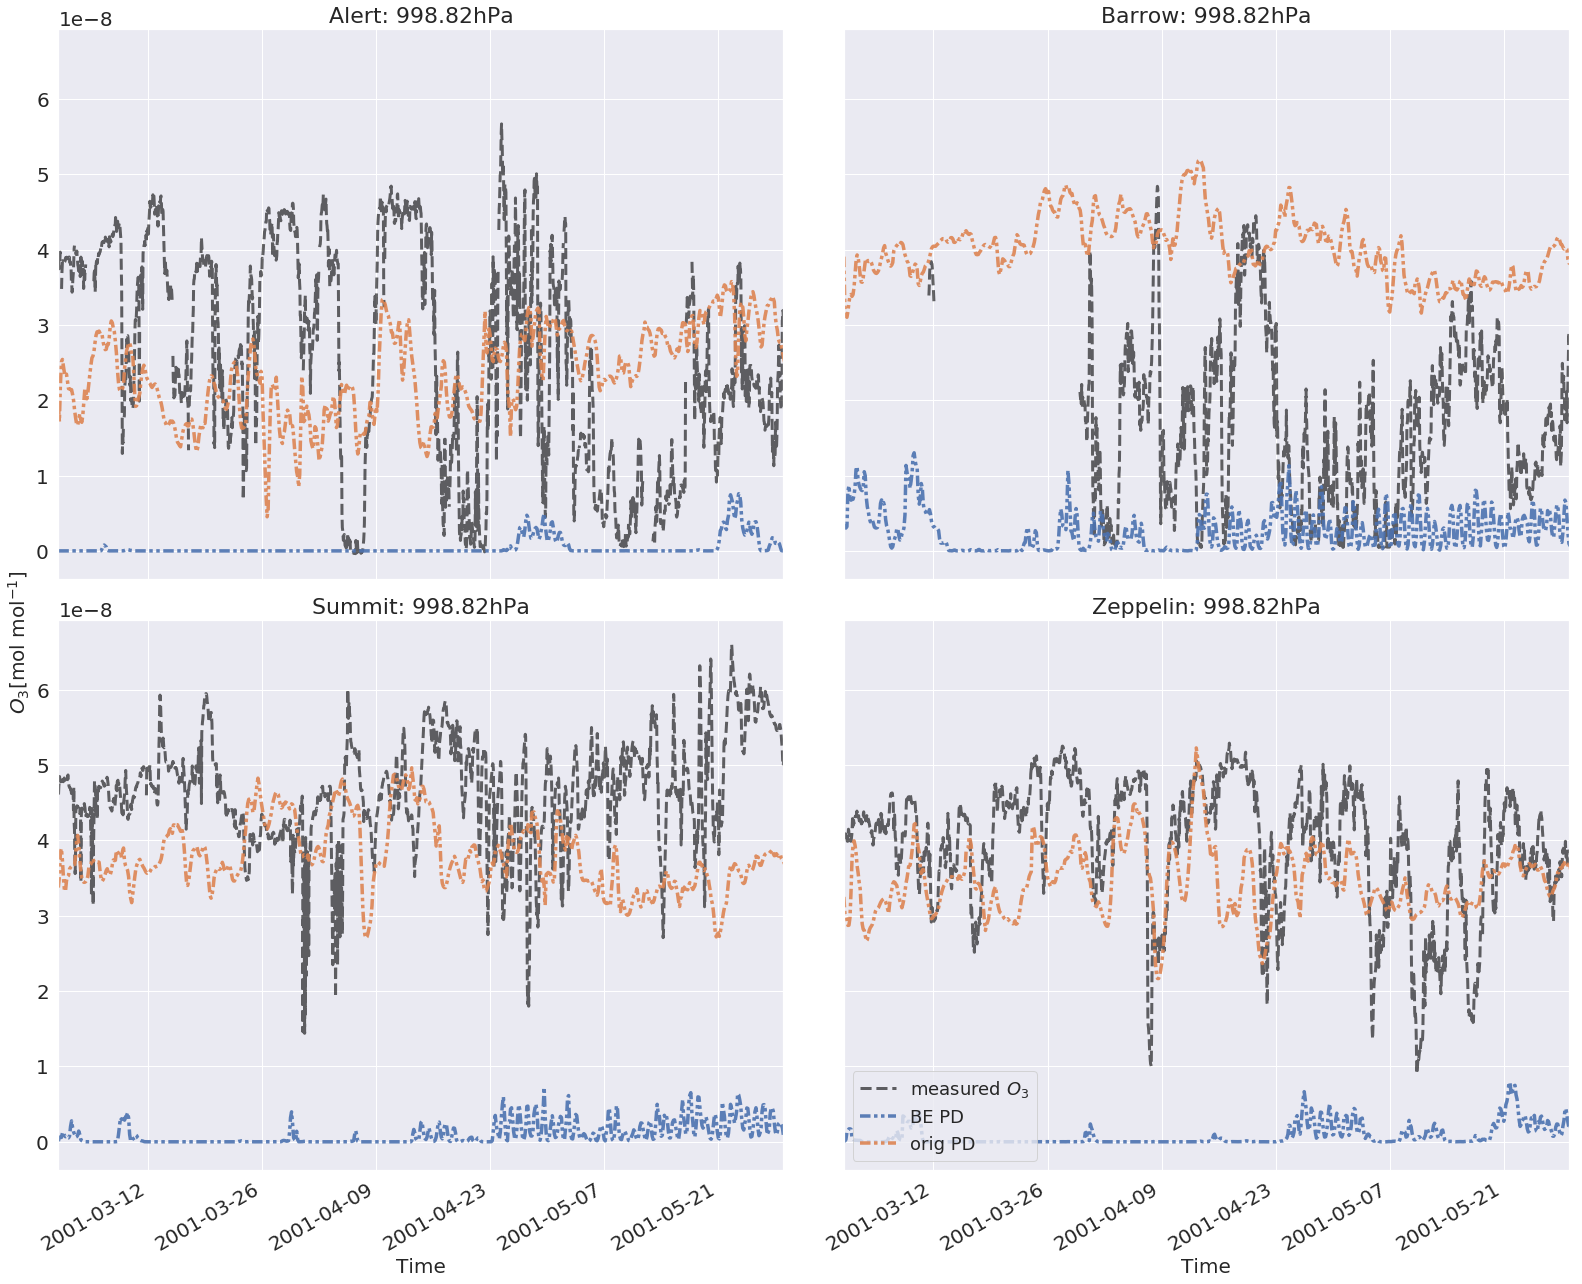
\includegraphics[width = \linewidth]{Chapter6_Results/images/ozone_2001_compObsOrigBE.png}
    \caption{Caption}
    \label{fig:CompObsOrigBE}
\end{figure}


\section{Test: Removing Heterogeneous Reactions}

Figure \ref{fig:test_RemoveHetReacts} shows results in terms of $\chem{O_3}$-concentration from attempting to turn off different heterogeneous reactions, namely snow/ice reactions (described in Section \ref{sec:snow_ice_react}), heterogeneous reactions over aerosol surfaces (described in Section \ref{sec:aerosol_react}) as well as heterogeneous reactions involving chlorine and bromine, respectively. The runs were initiated with the same restart file (spin-up) as Branch \ref{def:BE_PD}. For this purpose, four new branches were created (for a full overview of the branches, see Table \ref{tab:branches}). These were:

\begin{mydef}\label{def:BE_PD_noAerosol}
    \texttt{marikoll\_bromine\_explosion\_noHetAerosol}: Branch \ref{def:BE_PD} without heterogeneous aerosol reactions.
\end{mydef}

\begin{mydef}\label{def:BE_PD_noIce}
    \texttt{marikoll\_bromine\_explosion\_noSnowIce}: Branch \ref{def:BE_PD} without heterogeneous snow/ice reactions.
\end{mydef}

\begin{mydef}\label{def:BE_PD_noCl}
    \texttt{marikoll\_bromine\_explosion\_noHetChlorine}: Branch \ref{def:BE_PD} without heterogeneous reactions involving chlorine.
\end{mydef}

\begin{mydef}\label{def:BE_PD_noBr}
    \texttt{marikoll\_bromine\_explosion\_noHetBromine}: Branch \ref{def:BE_PD} without heterogeneous reactions involving bromine.
\end{mydef}


\begin{table}
\centering
\begin{tabular}{|ll|}
\hline
\textbf{Branch}                                      & \textbf{Reference}          \\ \hline
\texttt{marikoll\_originalCTM3\_NoStrat}             & \ref{def:origCTM3_PD}     \\
\texttt{marikoll\_originalCTM3\_noStrat\_pi}         & \ref{def:origCTM3_PI}     \\
\texttt{marikoll\_bromine\_explosion\_susanne}       & \ref{def:BE_PD}           \\
\texttt{marikoll\_bromine\_explosion\_PI}            & \ref{def:BE_PI}           \\
\texttt{marikoll\_bromine\_explosion\_noHetAerosol}  & \ref{def:BE_PD_noAerosol} \\
\texttt{marikoll\_bromine\_explosion\_noSnowIce}     & \ref{def:BE_PD_noIce}     \\
\texttt{marikoll\_bromine\_explosion\_noHetChlorine} & \ref{def:BE_PD_noCl}      \\
\texttt{marikoll\_bromine\_explosion\_noHetBromine}  & \ref{def:BE_PD_noBr}      \\ \hline
\end{tabular}
\caption{Overwiew of brances used in the developing process. References refer to chapter and branch number}
\label{tab:branches}
\end{table}


\begin{figure}
    \centering
    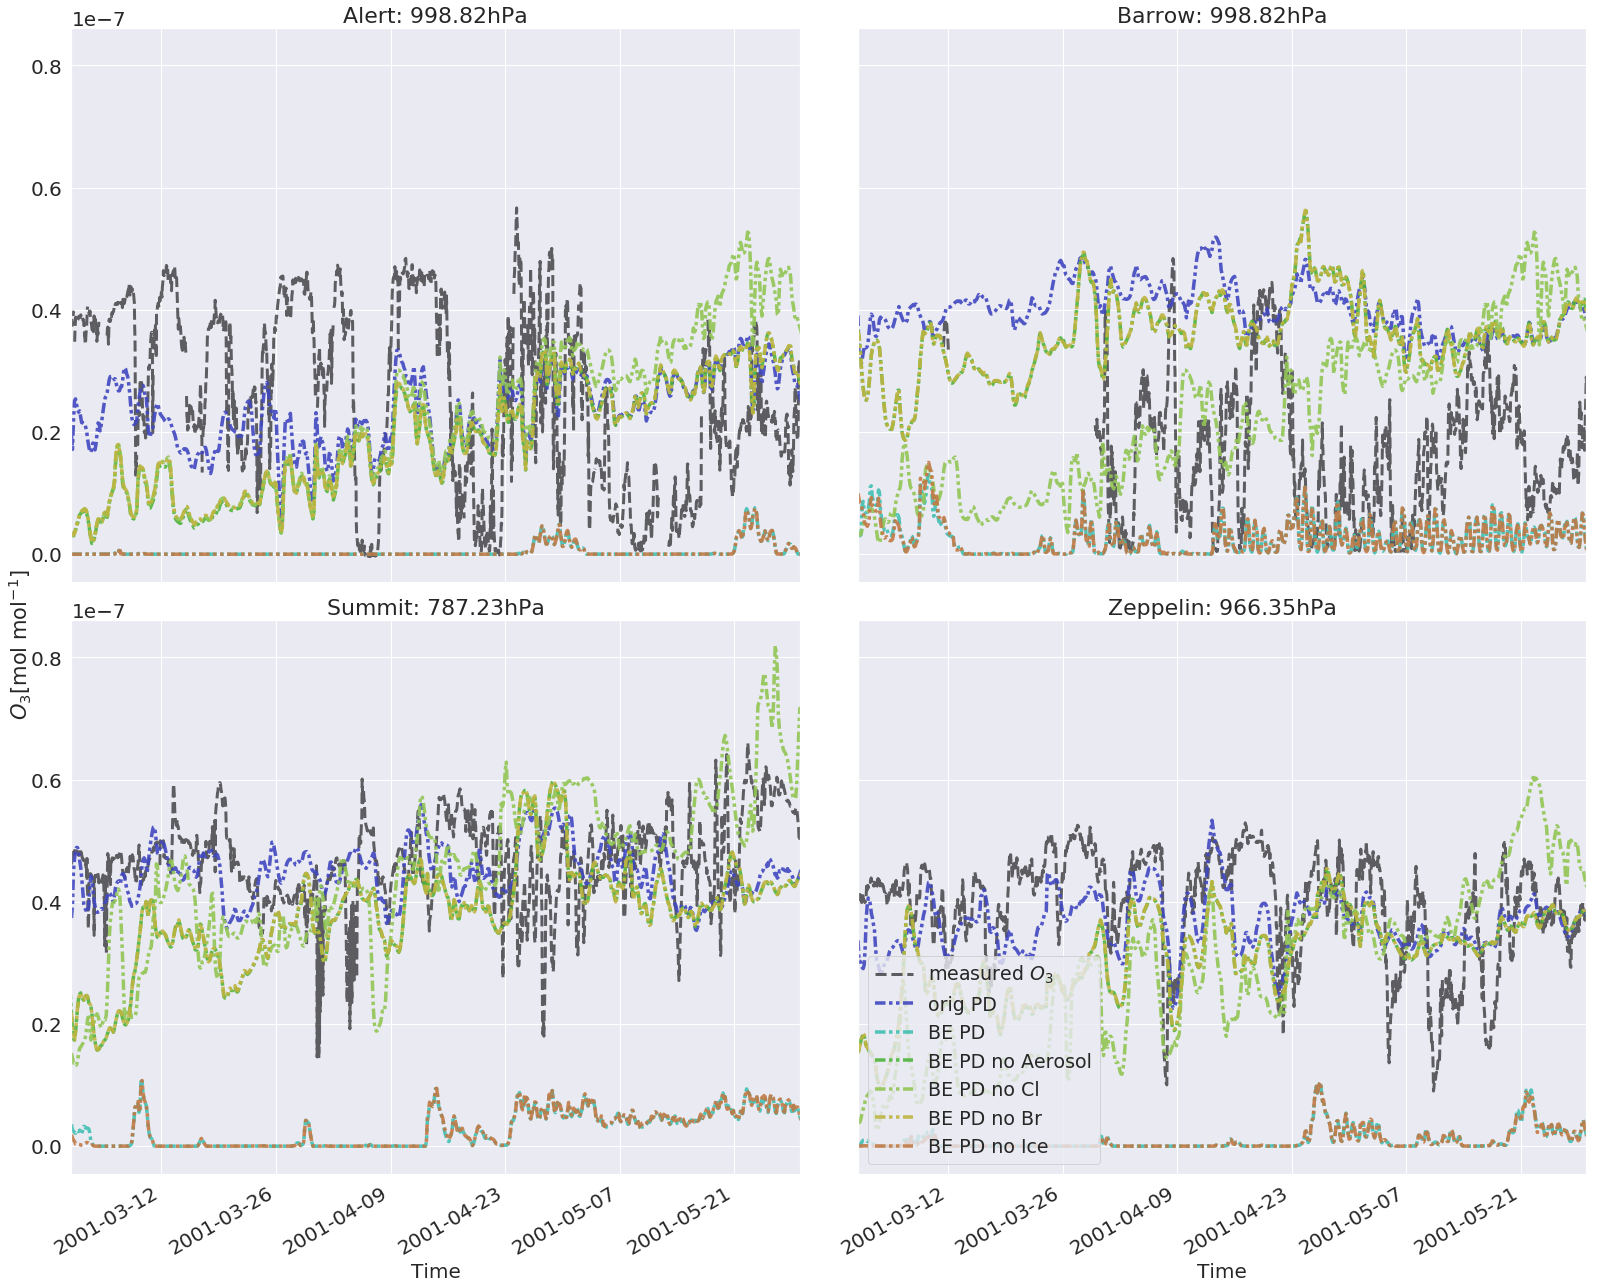
\includegraphics[width = \linewidth]{Chapter6_Results/images/ozone_removingHetReacts.png}
    \caption{Ozone measurements (black line) and model results from the original CTM3 (blue line), Branch \ref{def:BE_PD} (turquoise line), Branch \ref{def:BE_PD_noAerosol} (green line), \ref{def:BE_PD_noIce} (orange line), Branch \ref{def:BE_PD_noCl} (light green line) and Branch \ref{def:BE_PD_noBr} (yellow line) at the four different stations, Alert (top left), Barrow (top right), Summit (lower left) and Zeppelin (lower right) with available measurements in 2001. Model results were taken from the approximate altitude of the station in hPa. PD = present day, BE = bromine explosion}
    \label{fig:test_RemoveHetReacts}
\end{figure}


\medskip

In the vertical, the corresponding $\chem{Br_y}$ concentrations to Figure \ref{fig:test_RemoveHetReacts} are shown in Figures \ref{fig:vert_noAer_bry_2001}-\ref{fig:vert_noBr_bry_2001} for the four new branches, Branch \ref{def:BE_PD_noAerosol}-\ref{def:BE_PD_noBr}, respectively (The $\chem{Br_y}$-family is explained in Section \ref{sec:halogen_families_BryClxCly}). 

\begin{figure}
    \centering
    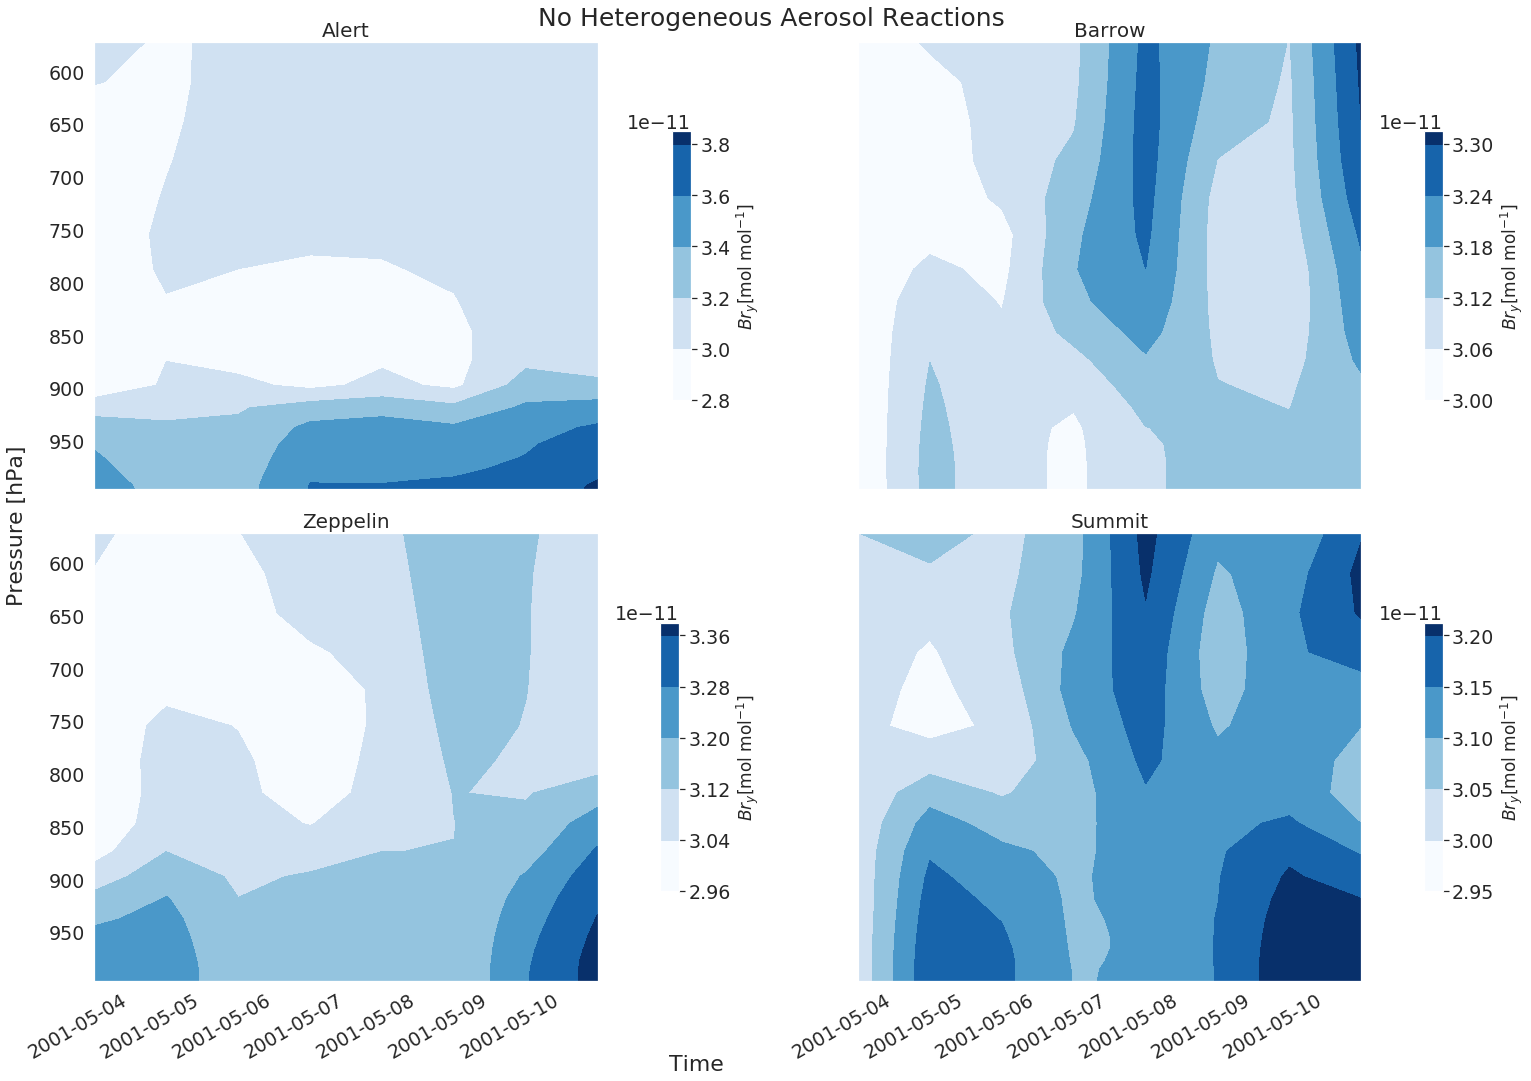
\includegraphics[width = \linewidth]{Chapter6_Results/images/noAerosol_2001_bry.png}
    \caption{Modelled $\chem{Br_y}$ without the heterogeneous aerosol reactions. The y-axis shows altitude up to 600 hPa at each station with ozone measurements at 12:00 (UTC) (Alert, Barrow, Zeppelin and Summit) in 2001.}
    \label{fig:vert_noAer_bry_2001}
\end{figure}

\begin{figure}
    \centering
    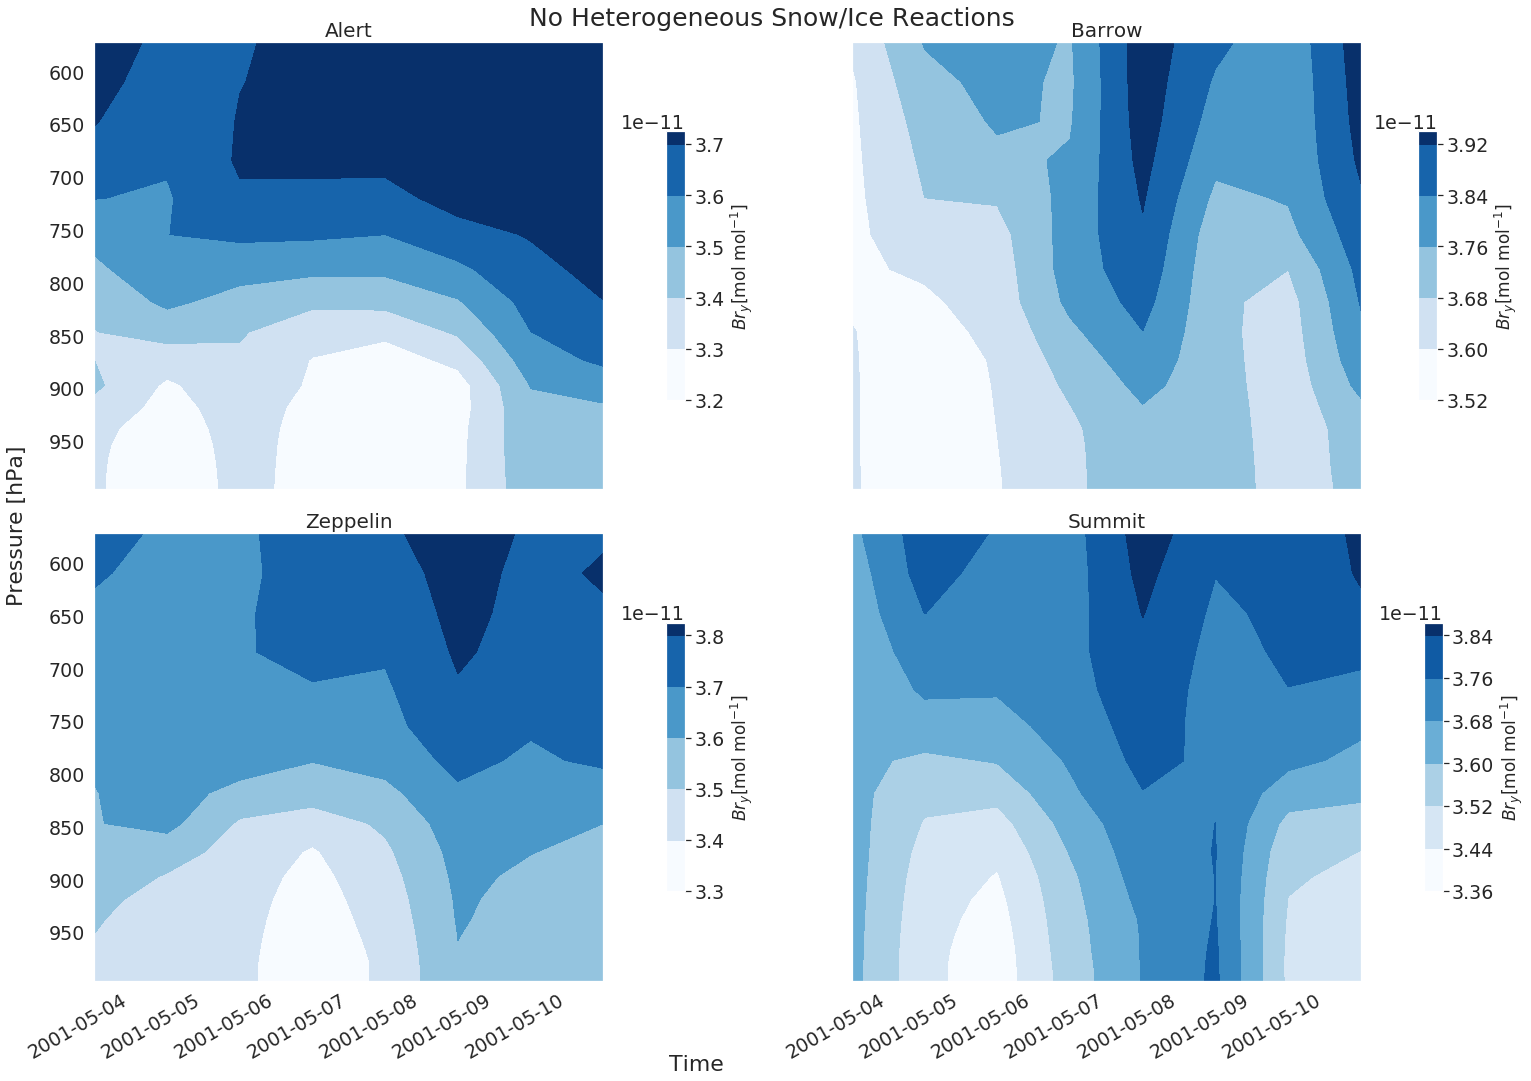
\includegraphics[width = \linewidth]{Chapter6_Results/images/noSnowIce_2001_bry.png}
    \caption{Modelled $\chem{Br_y}$ without theheterogeneous reactions over ice surfaces. The y-axis shows altitude up to 600 hPa at each station with ozone measurements (Alert, Barrow, Zeppelin and Summit) in 2001.}
    \label{fig:vert_noSnowIce_bry_2001}
\end{figure}

\begin{figure}
    \centering
    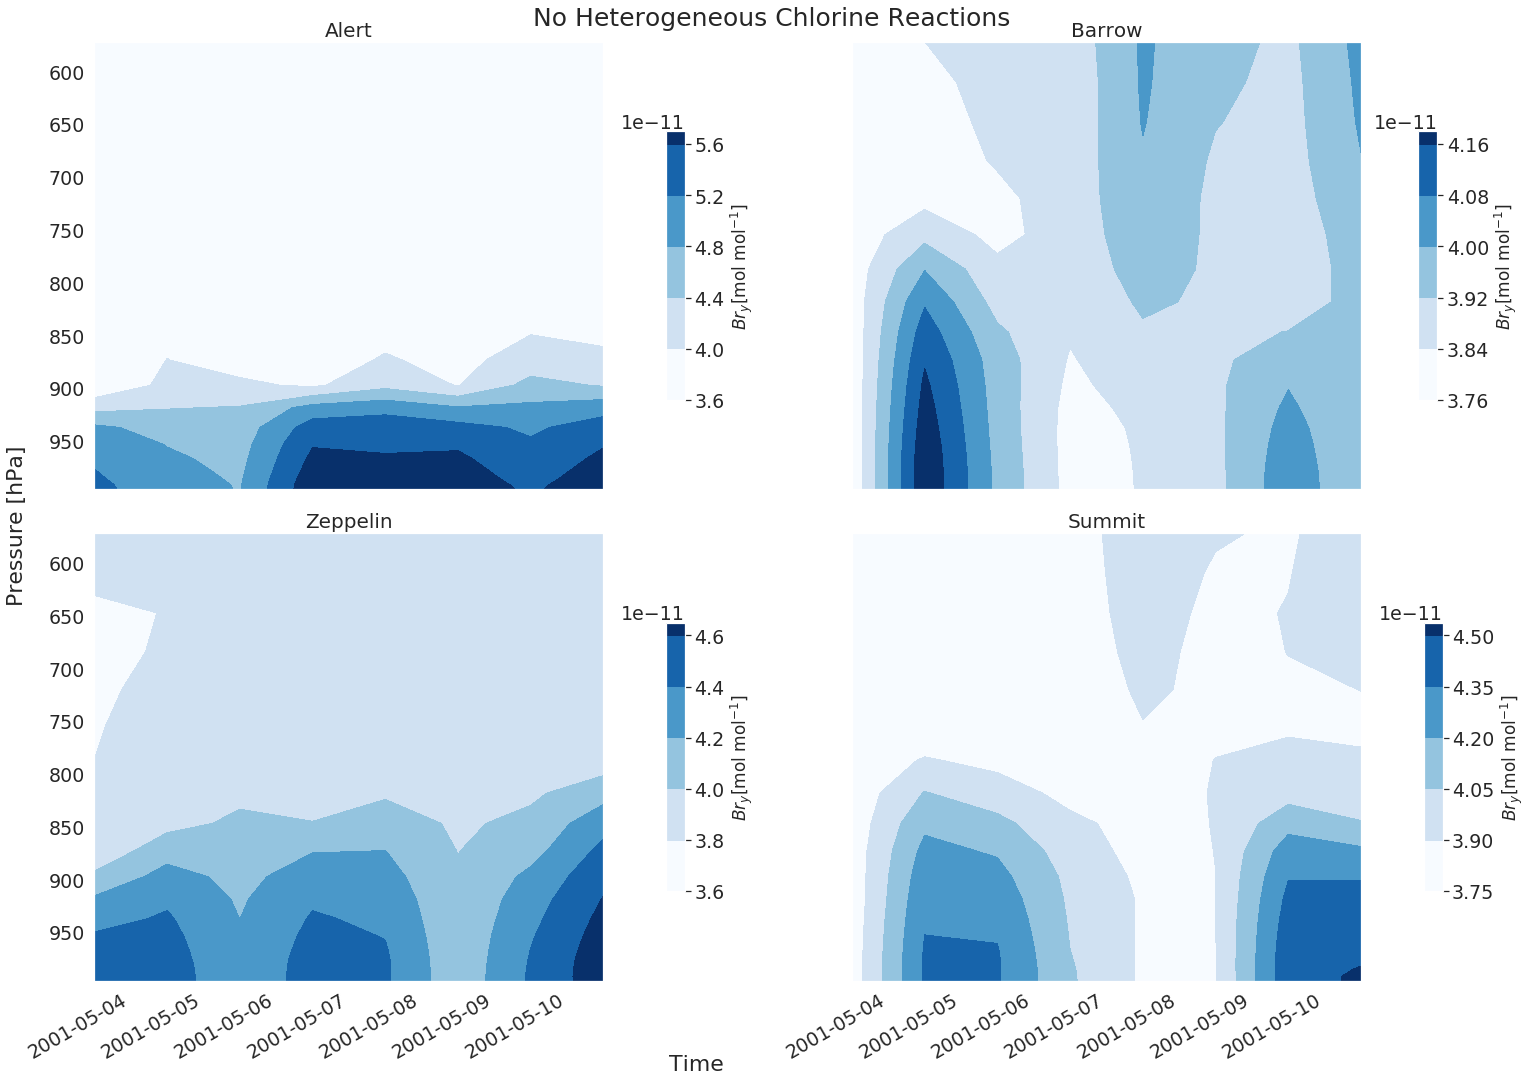
\includegraphics[width = \linewidth]{Chapter6_Results/images/noCl_2001_bry.png}
    \caption{Modelled $\chem{Br_y}$ without the heterogeneous reactions involving chlorine. The y-axis shows altitude up to 600 hPa at each station with ozone measurements (Alert, Barrow, Zeppelin and Summit) in 2001.}
    \label{fig:vert_noCl_bry_2001}
\end{figure}

\begin{figure}
    \centering
    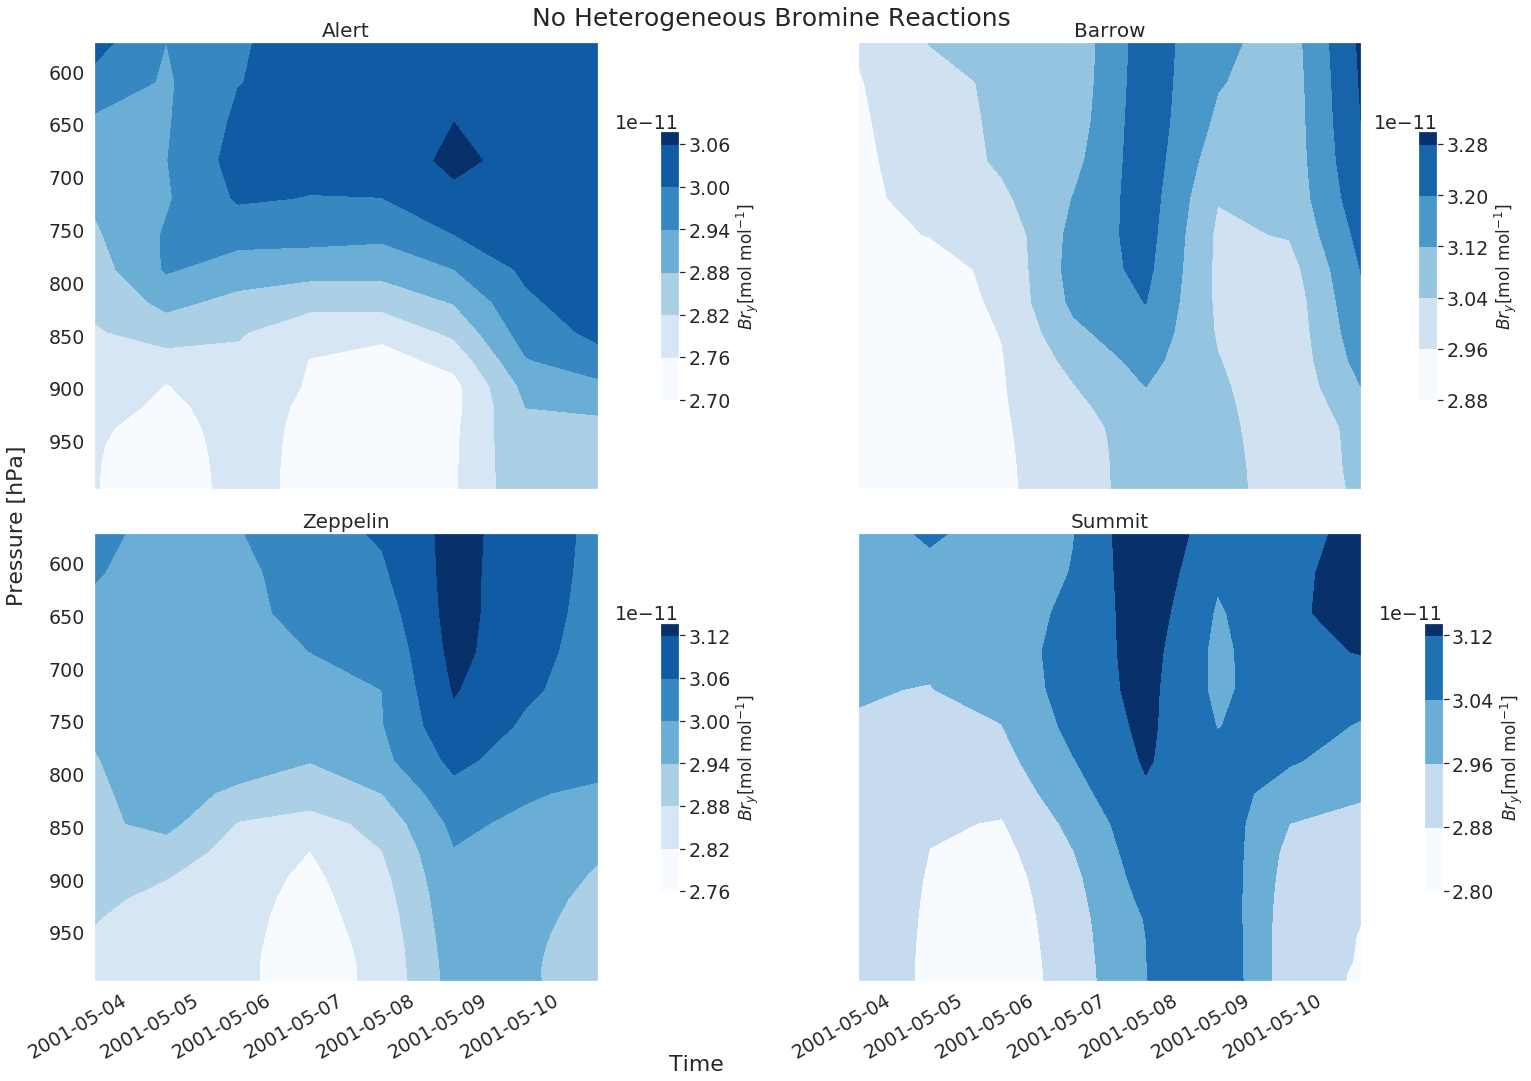
\includegraphics[width = \linewidth]{Chapter6_Results/images/noBr_2001_bry.png}
    \caption{Modelled $\chem{Br_y}$ without the heterogeneous reactions involving bromine. The y-axis shows altitude up to 600 hPa at each station with ozone measurements at 12:00 (UTC) (Alert, Barrow, Zeppelin and Summit) in 2001.}
    \label{fig:vert_noBr_bry_2001}
\end{figure}




\textbf{NOTE:} after these tests, a mistake in the scaling of $\chem{Cl_x}$ was discovered. \chem{BrCl} had mistakenly been scaled with this family, which led to disappearance of all \chem{Cl}-species. The subsequent tests were fixed for this.

\subsection{Integrating $\chem{Cl_y}$}

Figure \ref{fig:test_ClyInt} contains the result in terms of $\chem{O_3}$ concentration where an integration of the $\chem{Cl_y}$-family was added. This integration was not handled prior to the previous model runs (the chemical families are listed in Section \ref{sec:halogen_families_BryClxCly}). 

\medskip

As the inclusion of $\chem{ClONO2}$ (Reaction \ref{R:clono2}) function purely as a sink to the $\chem{ClO}$, this reaction was also removed altogether to see if this would help the low chlorine levels. 

\begin{figure}
    \centering
    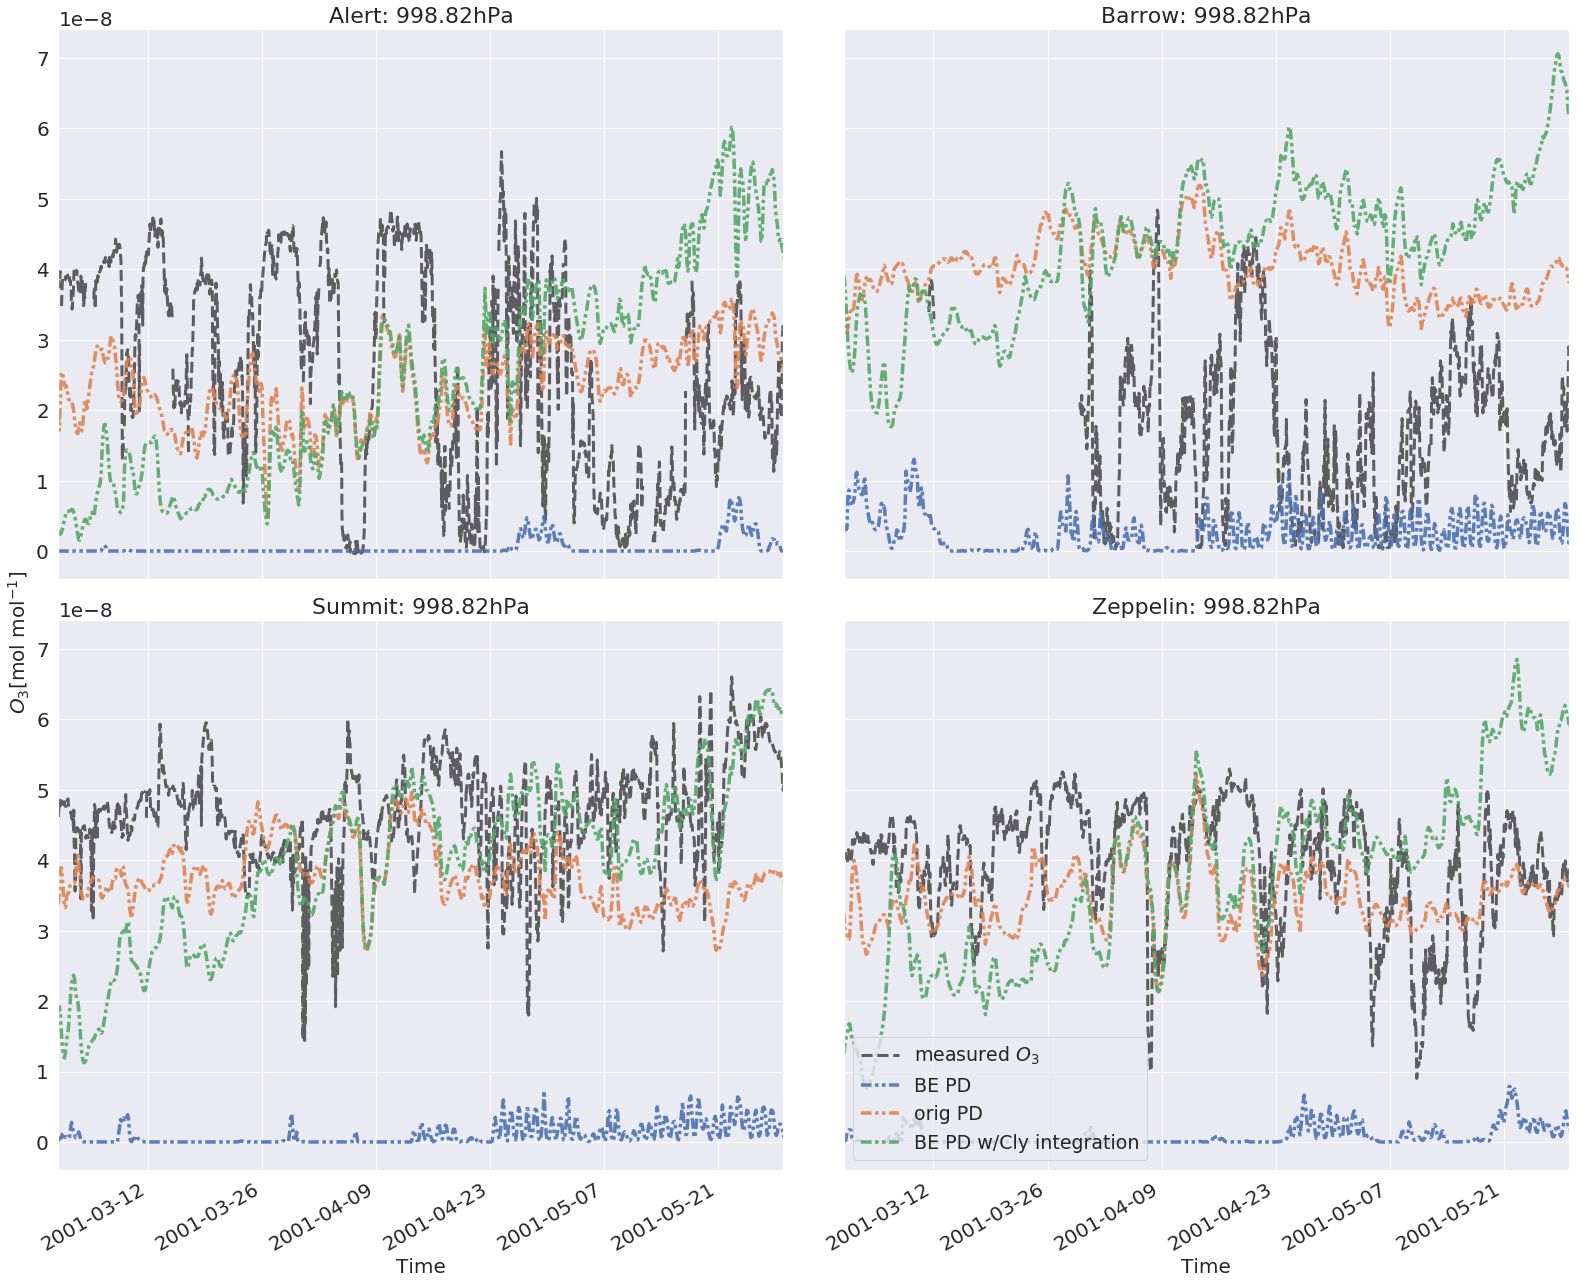
\includegraphics[width = \linewidth]{Chapter6_Results/images/ozone_2001_newClyIntegration.png}
    \caption{Ozone measurements (black line) and model results from the original CTM3 (orange line), Branch \ref{def:BE_PD} (blue line) and the attempt to integrate the $\chem{Cl_y}$ family (green line) at the four different stations, Alert (top left), Barrow (top right), Summit (lower left) and Zeppelin (lower right) with available measurements in 2001. Model results are taken from the first model level at $998.82 hPa$. PD = present day, BE = bromine explosion}
    \label{fig:test_ClyInt}
\end{figure}

\subsection{Changing $L_{mix}$ in Reaction \ref{R:7}}

The boundary layer height, $L_{mix}$ and deposition velocity, $v_d$ in the preliminary runs had values listed in Section \ref{sec:impl_multiphase_react}. In an attempt to "kick-start" the bromine explosions $L_{mix}$ was lowered (And corresponding $v_d$ increased) in the \texttt{marikoll\_bromine\_explosion\_noHetChlorine}- branch. 

\medskip

The first test was executed with $L_{mix} = 25 m$ and $v_d = 0.00824 m/s$. This boundary layer height was chosen due to the height of the second model layer height $995.86 hPa$, with is about $23 m$ higher than the first model layer height at $998.82 hPa$. The low level was chosen to make sure the bromine explosion would indeed occur. This test caused too much bromine explosion for the model to complete the run. $L_{mix}$ was then lowered to $L_{mix} = 100 m$ with $v_d = 0.00667 m/s$. 


\section{Comparison between the PD- and PI-branches}

\section{Comparison with station data}

\section{Comparison with literature}

Measurements of $\chem{Br_2}$, \chem{BrCl} and $\chem{O_3}$ were conducted by \cite{Foster2001} at Alert research station. They found $\chem{Br_2}$ mixing ratios up to $\sim$ 25 \acrshort{ppt} and \chem{BrCl} at mixing ratios up to 35 \acrshort{ppt} between day 40 and 75 in 2001. Ozone was depleted from background values of $\sim$ 30-40 \acrshort{ppb} to below 10 ppb. 

\medskip

\cite{Simpson2017} investigated the \chem{BrO} column using \acrlong{maxdoas} instrumentation near Barrow in 2012.

\medskip

\cite{Luo2018} also investigated the \chem{BrO} column using \acrshort{maxdoas} in Ny Ålesund in 2015. 

\medskip

\cite{Thomas2012} and \cite{Thomas2011} about the mechanism behind ODEs at Summit, Greenland. 

\section{Calculation of radiative forcing using PD- and PI model results}